% 2019-02-08

\documentclass[10pt]{article}
\usepackage[T1]{fontenc}
\usepackage{amssymb}
\usepackage{amsmath}
\usepackage{graphicx}
% \begin{figure}[h]
% \centering
% \includegraphics[width=6.5in]{folder/photo.png}
% \caption{}
% \label{}
% \end{figure}



\usepackage{tikz}
\usetikzlibrary{arrows}
\usepackage{subfigure}
\usepackage{stackrel}
\usepackage{blindtext}

\usepackage[url=false]{biblatex}
\addbibresource{library.bib}

\oddsidemargin=0.15in
\evensidemargin=0.15in
\topmargin=-.5in
\textheight=9in
\textwidth=6.25in

\usepackage[colorlinks=true,breaklinks,pdfpagemode=none,linkcolor=blue,citecolor=blue]{hyperref}

\usepackage{enumerate}
% \vspace{-6pt}
% \begin{itemize}
%     \setlength{\itemsep}{0pt}%
%     \setlength{\parskip}{0pt}%
%     \item Item 1
%     \item Item 2
%         \begin{itemize}
%             \setlength{\itemsep}{0pt}%
%             \setlength{\parskip}{0pt}%
%             \item Sublist Item 1
%             \item Sublist Item 2
%         \end{itemize}
%         \item Item 3
% \end{itemize}
% \vspace{-6pt}


\usepackage{enumitem}
\setlist{itemsep=0mm}

\usepackage{amsmath,amsfonts,amssymb,bm}


\begin{document}

   \noindent
   \begin{center}

   \hrulefill
   
   \vspace{5pt}
   
   \makebox[\textwidth]{ {\bf Energy Systems Analysis} \hfill  A.D. Smith 2019}
   \vspace{0pt}
   
   {\Large \hfill  Lecture 13. BEM: Building Systems, Part II\\ \hfill {\large Heating, Ventilation, \& Air Conditioning}}
   \vspace{5pt}
   
  
   \hrulefill
   \end{center}

   {\color{darkgray}{{\center{ \small{      ``A study of 60 buildings by Lawrence Berkeley 
National Laboratory showed that, before intervention, at least half had problems with their system 
controls, a minimum of 40\% had faulty HVAC equipment, and 25\% or more had problems with specific  `green' HVAC features (Piette, Nordman, & Greenberg, 1994). One group of researchers estimated that  finding and fixing these types of problems can save \$18 billion or more per year in commercial buildings  in the U.S. alone (Mills et al., 2004).''
\\%[3pt]
\rightline{{\rm --- Samuelson, Ghorayshi, and Reinhart \cite{Samuelson2016-ml}}}}}}}}


\section{EnergyPlus}

To allow EnergyPlus to incorporate HVAC equipment, we need to provide it with information about \cite{EPcourseteaching}:

\vspace{-6pt}
\begin{itemize}
    \setlength{\itemsep}{0pt}%
    \setlength{\parskip}{0pt}%
    \item Equipment types
    \item Operating schedules
    \item Control information
\end{itemize}
\vspace{-6pt}

There are many more types of HVAC systems than we could hope to cover, even having an entire semester to study HVAC. However, if you have a very basic amount of technical knowledge on a certain type of system, the Engineering Reference document \cite{EPdocs9engineering} contains the basic math describing how it's implemented in EnergyPlus. Unless your system is very unusual or new, it's likely someone has implemented it in EnergyPlus already. Figure \ref{vav} shows a simple abstracted illustration of a VAV system (Guest 1 Lecture), and the documentation explains the mathematical implementation of this system in EnergyPlus at the building level, zone level, and down to the coils in an individual VAV box \cite{EPdocs9engineering}. 

            \begin{figure}[h]
     \centering
            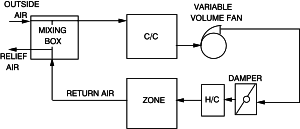
\includegraphics[width=3in]{extras13/VAVsys.png}
            \caption{Simplified Variable Volume Air System from EnergyPlus Engineering Reference \cite{EPdocs9engineering}}
            \label{vav}
            \end{figure}

\section{OpenStudio}

In OpenStudio, the HVAC Systems tab shows us a representation of the air systems distributing air through a building, or other "plant loops" circulating fluids (e.g. hot water or chilled water) within the building. In this tab, we can leverage templates that are already compiled (e.g. BCL \cite{BCL} or libraries added through File -> Load Library), which gives us a lot of drag \& drop functionality and ways to quickly set up HVAC systems. 

We have three sub-tabs within the right panel: 

\begin{description}
    \item[My Model] displays items that are part of your model already. \cite{OSdocs}
    \item[Library] includes components and measures that come with the application or are downloaded from the Building Component Library (BCL). \cite{OSdocs}
    \item[Edit] allows you to select certain components and edit the settings for that component. It is used in the HVAC tab to edit component settings, assign thermal zones to loops, and to add plenums. \cite{OSdocs}
\end{description}

\noindent
The ``Creating Your Model'' page in the OpenStudio documentation \cite{OSdocs} shows examples of your options for air and plant loops in the OpenStudio interface--click on \href{http://nrel.github.io/OpenStudio-user-documentation/tutorials/creating_your_model/#air-plant-and-zone-hvac-systems}{Air, Plant and Zone HVAC Systems}.

\section{Ventilation}

The EnergyPlus documentation defines ventilation and explains the minimum information needed to model it:

\begin{quote}
    \textbf{Ventilation} (Object: ZoneVentilation:DesignFlowRate) is the purposeful flow of air from the outdoor
environment directly into a thermal zone in order to provide some amount of non-mechanical
cooling \ldots Simple ventilation in EnergyPlus can be controlled by a schedule and through the
specification of minimum, maximum and delta temperatures. \cite{EPdocs9engineering}
\end{quote}

The outdoor air used for ventilation can be quantified by \cite{noauthor_undated-io}: 

\vspace{-6pt}
\begin{itemize}
    \setlength{\itemsep}{0pt}%
    \setlength{\parskip}{0pt}%
    \item CFM (cubic feet per minute) per person
    \item CFM per square foot (area) of the space
    \item Air Changes per Hour (ACH)
    \item Percent of total supply air
    \end{itemize}
    \vspace{-6pt}

The collections of fans, heating and cooling coils, and terminal units shown in OpenStudio's HVAC tab make up an air loop:

\begin{quote}
       In EnergyPlus an \textbf{air loop} is a central forced air HVAC system. The term `loop' is used because
in most cases some air is recirculated so that the air system forms a fluid loop. The air loop is
just the `air side' of a full HVAC system. The input objects related to these air loops begin
`AirLoopHVAC.'
For simulation purposes the air loop is divided into 2 parts: the primary air system (representing
the supply side of the loop) and the zone equipment (representing the demand side of the loop).
\end{quote}

 

When we talk about ventilation, we also have to acknowledge \textbf{infiltration}, which is ``air leakage'' or more generally any air flow to the interior that isn't directed by design (such as through mechanical systems bringing air in through an air handling unit). This needs to be included in the model for the airflow and overall heat balance models to be correct.

% \vspace{-6pt}
% \begin{itemize}
%     \setlength{\itemsep}{0pt}%
%     \setlength{\parskip}{0pt}%
%     \item Intent is to allow simple mechanical ventilation without specifying an HVAC system or natural ventilation
%     \item Amount of ventilation determined by user defined design flow rate, schedule, and equation similar to infiltration (allows for variation based on temperature difference and wind speed)
%     \item Type and control of ventilation determined by ventilation specific parameters
% \end{itemize}
% \vspace{-6pt}


\section{Sizing HVAC equipment}

EnergyPlus has a ``sizing manager'' module that can do sizing calculations for equipment, including some newer advanced options for HVAC equipment. The general method includes \cite{EPdocs9engineering}:

\begin{quote}
\begin{enumerate}
    \item A zone by zone heat balance load and air-flow calculation for multiple design days;
    \item Significant user control with modest input requirements;
    \item Zone, system and plant level calculations of design heating and cooling capacities and fluid
flow rates;
\item Modular, component-specific sizing algorithms for each HVAC component.
\item Options for monitoring how the initial sizes operate over multiple design days and then making
adjustments and repeating plant level calculations
\end{enumerate}
\end{quote}

\section{Controls and temperature setpoints}

EnergyPlus has many ways to implement control of HVAC systems, some of which might correspond directly to an actual piece of equipment that implements control logic, and some which are more abstract or much more high-level. One simple type of control which you will be familiar with and may interact with in your simulation models is the thermostat controlling a zone. Because a zone is assumed to be at uniform temperature (Lecture 12), this is the most detailed level of thermostat control that's possible. 

This is managed in EnergyPlus using the ZoneControl:Thermostat object, which has a few valid types of control: 

\begin{description}
\item[0] Uncontrolled (No specification---temperature will be determined using energy balances but the equipment will not attempt to reach or maintain a temperature)
\item[1] Single Heating Setpoint (No cooling specification)
\item[2] Single Cooling SetPoint (No heating specification)
\item[3] Single Heating/Cooling Setpoint (Same setpoint whether in heating or cooling mode)
\item[4] Dual Setpoint (Heating and Cooling) with deadband
\end{description}


\section{Heating}

Here are a few types of equipment that you may see in HVAC models for heating \cite{EPdocs9inputoutput}:

\begin{quote}
\begin{description}
\item[Baseboard Heat] baseboard heating system, controlled by a thermostat and heated with hot water or electric resistance heating.
\item[Heat Pump] generic term for a device that moves heat from a cold source to a hot sink---like a refrigerator, but we're interested in $Q_H$ instead of $Q_L$ \cite{cengel}.
\item[Boiler] heating device that heats up water to provide thermal energy, often by burning natural gas
\item[Furnace] heating device that heats up air, often by burning natural gas
\end{description}
\end{quote}


 \section{Cooling}

Here are a few types of equipment that you may see in HVAC models for cooling \cite{EPdocs9inputoutput}:

\begin{quote}
\begin{description}
\item[Chiller] generic term for a device that removes heat from a liquid, often water
\item[Vapor-compression chiller] a chiller that operates on the vapor-compression refrigeration cycle (and here we care about $Q_L$)
\item[Chilled beam]  a heat exchanger at ceiling level, as seen in the MEK building. Basic idea: 
\begin{quote}
    Warm air from the
space rises toward the ceiling, and the
air surrounding the chilled beam is
cooled, causing it to descend back
toward the floor, creating convective air
motion to cool the space. This allows a
passive chilled beam to provide space
cooling without the use of a fan. \cite{Murphy2009-un}
\end{quote}


\end{description}
\end{quote}



\section{Ideal System Air Loads}

EnergyPlus has a useful capability to study the ``loads'' or demands on an HVAC system without being tied a given type of system. This is handled within the ZoneHVAC:IdealLoadsAirSystem object.

\begin{quote}
    It is not connected
to a central air system---instead each ZoneHVAC:IdealLoadsAirSystem object supplies cooling or
heating air to a zone in sufficient quantity to meet the zone load or up to its limits, if specified \ldots It is modeled as an ideal VAV terminal unit with variable
supply temperature and humidity. The supply air flow rate is varied between zero and the maximum
in order to satisfy the zone heating or cooling load, zone humidity controls, outdoor air requirements,
and other constraints, if specified.
\cite{EPdocs9engineering}
\end{quote}

Note that because it's ``ideal'' you won't get proper quantification of the costs and needs of an actual HVAC system (e.g. fan energy, electricity or fuel costs).

\begin{quote}
The energy required to condition the supply air is metered and reported as DistrictHeating and DistrictCooling. \cite{EPdocs9inputoutput}
\end{quote}

% license
\bigskip

\noindent
\texttt{\footnotesize RESTRICTED PUBLIC LICENSE --- READ BEFORE SHARING. This is a draft version made available by Amanda D. Smith under a Creative Commons Attribution-NonCommercial-ShareAlike license. 
\href{https://creativecommons.org/licenses/by-nc-sa/4.0/}{CC BY-NC-SA 4.0}}

% references

\printbibliography

\end{document}